\documentclass[sigconf]{webmedia}
%webmeda.cls is adapted from acmart.cls for use in Proceedings of the Brazilian Symposium on Multimedia and the Web (WebMedia)

\usepackage{lmodern}
% Com o webmedia.cls (que carrega newtxmath) + lmodern, ( ) [ ] + = / < > etc. em modo matematico
% apontam para posicoes inexistentes nas fontes do Latin Modern e somem do PDF. Estas linhas
% devolvem os caracteres ASCII de modo matematico as definicoes do LaTeX padrao (fontmath.ltx).
\DeclareMathDelimiter{(}{\mathopen}{operators}{"28}{largesymbols}{"00}
\DeclareMathDelimiter{)}{\mathclose}{operators}{"29}{largesymbols}{"01}
\DeclareMathDelimiter{[}{\mathopen}{operators}{"5B}{largesymbols}{"02}
\DeclareMathDelimiter{]}{\mathclose}{operators}{"5D}{largesymbols}{"03}
\DeclareMathDelimiter{/}{\mathord}{letters}{"3D}{largesymbols}{"0E}
\DeclareMathSymbol{+}{\mathbin}{operators}{"2B}
\DeclareMathSymbol{=}{\mathrel}{operators}{"3D}
\DeclareMathSymbol{<}{\mathrel}{letters}{"3C}
\DeclareMathSymbol{>}{\mathrel}{letters}{"3E}
\DeclareMathSymbol{:}{\mathrel}{operators}{"3A}
\DeclareMathSymbol{;}{\mathpunct}{operators}{"3B}
\DeclareMathSymbol{!}{\mathclose}{operators}{"21}
\DeclareMathSymbol{?}{\mathclose}{operators}{"3F}
\let\sum\relax
\DeclareMathSymbol{\sum}{\mathop}{largesymbols}{"50}
\usepackage[brazil]{babel}
\usepackage{booktabs}
\usepackage{multirow}
\setlength{\emergencystretch}{1.5em} % evita linhas alem da margem

\AtBeginDocument{%
  \providecommand\BibTeX{{%
    \normalfont B\kern-0.5em{\scshape i\kern-0.25em b}\kern-0.8em\TeX}}}

\settopmatter{printacmref=false, printfolios=false}
\setevent{webmedia}
\proceedingsDetails[WebMedia’2026]{Proceedings of the Brazilian Symposium on Multimedia and the Web}{2026}{Lavras/MG, Brazil}
\ISSN{2966-2753}

% todos os numeros do texto sao gerados por src/gerar_artigo.py a partir de results/
% gerado por src/gerar_artigo.py -- nao editar
\newcommand{\NVertices}{99.438}
\newcommand{\NArestas}{1.571.480}
\newcommand{\NUsuarios}{33.387}
\newcommand{\NCervejas}{66.051}
\newcommand{\NAvLidas}{1.586.614}
\newcommand{\NAvSemUsuario}{348}
\newcommand{\NParesRepetidos}{14.274}
\newcommand{\NAvFundidas}{14.786}
\newcommand{\DataDownload}{22/11/2026}
\newcommand{\NBytesBruto}{445.475.306}
\newcommand{\DataMin}{22/08/1996}
\newcommand{\DataMax}{11/01/2012}
\newcommand{\GrauMax}{5.782}
\newcommand{\GrauMedio}{31{,}61}
\newcommand{\GrauMedioU}{47{,}07}
\newcommand{\GrauMaxU}{5.782}
\newcommand{\GrauMedioB}{23{,}79}
\newcommand{\GrauMaxB}{3.206}
\newcommand{\FracGrauUm}{34{,}5\%}
\newcommand{\Densidade}{3{,}18\times 10^{-4}}
\newcommand{\DensidadeBip}{7{,}13\times 10^{-4}}
\newcommand{\NComponentes}{42}
\newcommand{\NCompPequenas}{41}
\newcommand{\MCCVertices}{99.356}
\newcommand{\MCCArestas}{1.571.439}
\newcommand{\MCCPercent}{99{,}92\%}
\newcommand{\Diametro}{9}
\newcommand{\Raio}{5}
\newcommand{\LExato}{3{,}725}
\newcommand{\FracDistAteQuatro}{86{,}9\%}
\newcommand{\TempoDistHoras}{1{,}1}
\newcommand{\BFSLimitantes}{38}
\newcommand{\Triangulos}{0}
\newcommand{\Clusterizacao}{0{,}0}
\newcommand{\VizVertices}{250}
\newcommand{\VizArestas}{436}
\newcommand{\DFSArvores}{42}
\newcommand{\TarjanCFC}{42}
\newcommand{\EulerImpares}{62.054}
\newcommand{\EulerImparesMCC}{61.972}
\newcommand{\AGMPeso}{177.260{,}33}
\newcommand{\BFPassadasUteis}{4}
\newcommand{\BFPassadasFaixa}{4}
\newcommand{\PBootLimite}{0{,}002}
\newcommand{\BFOrigens}{10}
\newcommand{\TrocasSobreposicaoEsperada}{15{,}6\%}
\newcommand{\BFTempoPassada}{0{,}281}
\newcommand{\EstBFHoras}{7{,}8}
\newcommand{\EstFWAnos}{1{,}0}
\newcommand{\FWnsOp}{33}
\newcommand{\EstFWMemGB}{79}
\newcommand{\TarjanArt}{7.260}
\newcommand{\TarjanPontes}{34.340}
\newcommand{\TarjanPontesFolha}{34.185}
\newcommand{\DijkstraMax}{16{,}0}
\newcommand{\DijkstraMedia}{5{,}51}
\newcommand{\ExpMin}{1{,}03}
\newcommand{\ExpMax}{1{,}18}
\newcommand{\ExpRepMin}{0{,}82}
\newcommand{\ExpRepMax}{1{,}04}
\newcommand{\ExpKruskal}{0{,}76}
\newcommand{\ExpKruskalRep}{1{,}00}
\newcommand{\KruskalNsMaior}{54}
\newcommand{\KruskalNsMCC}{29}
\newcommand{\ExpBF}{1{,}06}
\newcommand{\ExpBFRep}{1{,}02}
\newcommand{\ExpBFV}{3{,}03}
\newcommand{\ExpFW}{1{,}00}
\newcommand{\TempoBFS}{0{,}137}
\newcommand{\TempoDijkstra}{0{,}674}
\newcommand{\RazaoDijkstraBFS}{4{,}9}
\newcommand{\TempoTotalDesempenho}{16}
\newcommand{\LERformula}{3{,}33}
\newcommand{\CERformula}{3{,}18\times 10^{-4}}
\newcommand{\LERsim}{3{,}71}
\newcommand{\LatapyG}{0{,}0599}
\newcommand{\LatapyR}{0{,}0306}
\newcommand{\LatapyRazao}{1{,}96}
\newcommand{\LBipR}{3{,}672}
\newcommand{\RazaoL}{1{,}014}
\newcommand{\SigmaBip}{1{,}93}
\newcommand{\RTrocas}{10}
\newcommand{\QTrocas}{10}
\newcommand{\TrocasAceitasPct}{66{,}3\%}
\newcommand{\TrocasRestantesPct}{15{,}4\%}
\newcommand{\LatapyAmostra}{2.000}
\newcommand{\GrauMaxBA}{2.024}
\newcommand{\GammaTodos}{1{,}57}
\newcommand{\KminTodos}{2}
\newcommand{\KSTodos}{0{,}025}
\newcommand{\GammaU}{1{,}45}
\newcommand{\GammaB}{1{,}62}
\newcommand{\GammaTodosAprox}{1{,}554}
\newcommand{\GammaTodosExato}{1{,}565}
\newcommand{\BBoot}{500}
\newcommand{\PBootMax}{0{,}000}
\newcommand{\KSSintMax}{0{,}006}
\newcommand{\RobR}{4.968}
\newcommand{\RobN}{99.356}
\newcommand{\RobSAleat}{0{,}9832}
\newcommand{\RobBAleat}{1.577{,}7}
\newcommand{\RobDAleat}{1{,}66\%}
\newcommand{\RobCBase}{3{,}725}
\newcommand{\RobCAleat}{3{,}724}
\newcommand{\RobCAleatIC}{[3{,}708; 3{,}739]}
\newcommand{\RobSAlvo}{0{,}4341}
\newcommand{\RobBAlvo}{52.451}
\newcommand{\RobDAlvo}{54{,}7\%}
\newcommand{\RobCAlvo}{6{,}011}
\newcommand{\RobCAlvoIC}{[5{,}984; 6{,}038]}
\newcommand{\RobKAlvo}{2.000}
\newcommand{\RobGrauCorte}{136}
\newcommand{\RobEmpatesRem}{20}
\newcommand{\RobEmpatesTot}{33}
\newcommand{\Hardware}{Intel Core i5-12450H (8 núcleos, 12 threads), 15,7 GB de RAM}
\newcommand{\SO}{Windows 11 Home 64 bits}
\newcommand{\PythonVersao}{3.15.2}
\newcommand{\LinkRepositorio}{https://github.com/USUARIO/tp-grafos-g115}
\newcommand{\DeclaracaoIA}{Este trabalho foi desenvolvido com uso intensivo do assistente de programação Claude Code (Anthropic, modelo Claude Opus 5.5). A partir das instruções do autor, o assistente escreveu o código, executou os experimentos, gerou as figuras e redigiu o texto. O autor definiu os requisitos e as restrições do trabalho e escolheu, entre as alternativas apresentadas, a modelagem bipartida usuário--cerveja. Todos os números do texto são gerados automaticamente a partir dos arquivos de resultados do repositório. O autor é responsável pelo conteúdo entregue.}
\newcommand{\Descoberta}{A conectividade da rede depende de um núcleo pequeno de vértices. Os 4.968 vértices de maior grau (grau $\ge$ 136; 2.546 usuários e 2.422 cervejas) concentram 70{,}8\% da soma dos graus da MCC. Ao removê-los, 51.618 vértices (54{,}7\% dos restantes) ficam isolados, dos quais 38.721 são cervejas: todos os avaliadores dessas cervejas estão entre os 2.546 usuários removidos. Ou seja, a maior parte do catálogo só se liga ao restante da rede por meio de um grupo pequeno de usuários muito ativos.}


\begin{document}

\title{Análise Estrutural e Algorítmica do Grafo Bipartido Usuário--Cerveja do BeerAdvocate}
\subtitle{Trabalho Prático de MATA53 -- Teoria dos Grafos (UFBA) -- Grafo G115}

% o campo \email do template nao aceita acentos nem espacos; a matricula vai numa nota do autor
\author{Vinicius Schedler}
\authornote{Matrícula 223115843.}
\affiliation{%
  \institution{Universidade Federal da Bahia, Instituto de Computação}
  \city{Salvador}
  \state{BA}
  \country{Brasil}}

\renewcommand{\shortauthors}{V. Schedler}

\begin{abstract}
Este trabalho analisa o conjunto \textit{web-BeerAdvocate} do SNAP (grafo G115). Como o conjunto
é formado por avaliações, e não por uma lista de arestas, modelamos um grafo bipartido não
direcionado usuário--cerveja com \NVertices{} vértices e \NArestas{} arestas. Calculamos as
medidas estruturais pedidas, implementamos em Python os algoritmos da disciplina (BFS, DFS,
eulerianidade, Dijkstra, Bellman-Ford, Floyd-Warshall, Tarjan, Prim e Kruskal), validamos cada
um contra o NetworkX e medimos seus tempos com intervalos de confiança. Na maior componente
conexa, que contém \MCCPercent{} dos vértices, as distâncias são curtas (comprimento médio
\LExato{}, diâmetro \Diametro{}). Por ser bipartido, o grafo não tem triângulos, e o critério
\textit{small-world} do enunciado não se aplica; com a medida de agrupamento própria para grafos
bipartidos, o agrupamento é \LatapyRazao{} vezes o de um grafo aleatório com os mesmos graus. A
distribuição de graus tem cauda pesada, mas o teste de bondade de ajuste rejeita a lei de
potência pura. A rede tolera a remoção aleatória de 5\% dos vértices e se fragmenta quando os
5\% de maior grau são removidos.
\end{abstract}

\keywords{teoria dos grafos, grafos bipartidos, SNAP, small-world, lei de potência, robustez}

\maketitle

% ======================================================================
\section{Introdução}

O objetivo do trabalho é aplicar os conceitos de MATA53 a um grafo real: tratar os dados,
calcular propriedades estruturais, implementar os algoritmos estudados e interpretar os
resultados. O grafo foi determinado pela regra
$f(M) = (\text{soma dos dígitos de } M)\times(\text{últimos 2 dígitos de } M + 1) \bmod 129$.
Para $M = 223115843$, a soma dos dígitos é $2+2+3+1+1+5+8+4+3 = 29$ e os dois últimos
dígitos são $43$; logo $f(M) = 29 \times 44 \bmod 129 = 1276 \bmod 129 = 115$, isto é,
o grafo G115, que na planilha da disciplina corresponde ao conjunto \textit{web-BeerAdvocate}
do SNAP~\cite{snap,mcauley2012,mcauley2013}.

A Seção~\ref{sec:dados} descreve os dados e o tratamento; a Seção~\ref{sec:metodologia}, a
metodologia; a Seção~\ref{sec:resultados}, os resultados das Partes I, II e III; a
Seção~\ref{sec:discussao} discute limitações; e a Seção~\ref{sec:conclusao} conclui.

% ======================================================================
\section{Grafo original e tratamento}\label{sec:dados}

\subsection{Conjunto de dados}
O \textit{web-BeerAdvocate} reúne avaliações de cervejas publicadas no site BeerAdvocate.
Cada registro contém identificadores da cerveja e da cervejaria, estilo, teor alcoólico,
cinco notas (aparência, aroma, paladar, sabor e nota geral \texttt{overall}), o instante
da avaliação, o nome de perfil do usuário e o texto da avaliação~\cite{mcauley2012}.
Registramos três divergências entre o enunciado, a página do SNAP e o arquivo obtido:
\begin{enumerate}
  \item O conjunto \textbf{não é uma lista de arestas}: o grafo precisa ser construído a
  partir das avaliações (Seção~\ref{sec:modelagem}).
  \item A página do SNAP informa que, a pedido do BeerAdvocate, os dados não estão mais
  disponíveis, e não declara licença de uso. Mesmo assim, o arquivo \texttt{Beeradvocate.txt.gz}
  ainda era servido e foi baixado em \DataDownload{} (\NBytesBruto{} bytes; SHA-256 no
  repositório). O repositório não inclui o arquivo bruto, os textos nem os nomes de usuário.
  \item O arquivo contém \NAvLidas{} avaliações, enquanto a página informa 1.586.259; o número
  de usuários (\NUsuarios{}) e de cervejas (\NCervejas{}) coincide. As avaliações vão de
  \DataMin{} a \DataMax{}; a página indica início em jan./1998.
\end{enumerate}

\subsection{Modelagem e tratamento}\label{sec:modelagem}
Modelamos um \textbf{grafo bipartido não direcionado} $G=(U\cup B, E)$, em que $U$ é o
conjunto de usuários (campo \texttt{review/\allowbreak profileName}), $B$ o de cervejas (campo
\texttt{beer/\allowbreak beerId})
e $\{u,b\}\in E$ se o usuário $u$ avaliou a cerveja $b$. Essa é a estrutura presente nos dados;
uma projeção usuário--usuário exigiria escolher um limiar arbitrário de cervejas em comum e
geraria um grafo muito mais denso. A Tabela~\ref{tab:tratamento} resume o tratamento.

\begin{table}[t]
\caption{Tratamento aplicado aos dados (\texttt{preparar\_dados.py}).}
\label{tab:tratamento}
\footnotesize
\begin{tabular}{@{}p{5.6cm}r@{}}
\toprule
Etapa & Quantidade \\
\midrule
Avaliações lidas & \NAvLidas \\
Descartadas sem \texttt{profileName} & \NAvSemUsuario \\
Pares usuário--cerveja repetidos (multiarestas) & \NParesRepetidos \\
Avaliações fundidas ao tornar o grafo simples & \NAvFundidas \\
Arestas do grafo simples & \NArestas \\
Usuários $|U|$ / cervejas $|B|$ & \NUsuarios{} / \NCervejas \\
\bottomrule
\end{tabular}
\end{table}

As decisões foram: (i) descartar avaliações sem nome de usuário, pois não há como
identificar o vértice; (ii) converter o multigrafo em grafo simples, com uma aresta por par e a
média das notas \texttt{overall} do par; (iii) usar todo o período (grafo estático, união das
arestas no tempo); (iv) não há laços, pois toda aresta liga um usuário a uma cerveja; (v) nos
algoritmos ponderados, usar o peso $w(u,b) = 6 - \bar{o}(u,b) \in [1,6]$, em que $\bar{o}$ é a
nota média do par. O peso é positivo (requisito de Dijkstra) e torna ``mais curta'' uma aresta
bem avaliada; é uma convenção nossa, pois os dados não trazem distâncias.

% ======================================================================
\section{Metodologia}\label{sec:metodologia}

\subsection{Representação e implementação}
Usamos listas de adjacência, a representação indicada nos slides para grafos esparsos
($|E| \ll |V|^2$); a matriz de adjacência teria $|V|^2 \approx 10^{10}$ posições. Os
algoritmos foram escritos em Python puro, seguindo os pseudocódigos das aulas
(Tabela~\ref{tab:algoritmos}) e a mesma notação ($d[v]$, $f[v]$, $\pi[v]$, cores, $key[v]$,
\textsc{Relaxa}). DFS e Tarjan usam pilha explícita, porque a recursão do Python não suporta
$\sim\!10^5$ níveis; a ordem de visita é a mesma da versão recursiva. Como o \texttt{heapq} não
tem \textsc{DiminuirChave}, Dijkstra e Prim reinserem o vértice no heap e descartam as entradas
obsoletas; o heap passa a ter até $|E|$ entradas, e o custo continua $O((V+E)\log V)$, pois
$\log E \le 2\log V$.

O enunciado pede ``o algoritmo de Tarjan''. Implementamos as duas versões descritas por
Tarjan~\cite{tarjan1972}, ambas baseadas em uma única DFS e no valor $low[v]$:
(a) \textbf{componentes fortemente conexas (CFC)}, o problema que os slides resolvem com a DFS no
grafo e no transposto~\cite{cormen2009}; e (b) \textbf{pontos de articulação e pontes}, a versão
para grafos não direcionados~\cite{hopcroft1973}. Para aplicar (a) ao nosso grafo, cada aresta
$\{u,v\}$ vira os arcos $(u,v)$ e $(v,u)$. Nesse grafo dirigido simétrico, $u$ alcança $v$ se e
somente se $v$ alcança $u$, logo as CFC coincidem com as componentes conexas, e o resultado serve
como conferência. A versão (b) dá informação nova: quais vértices e arestas, se removidos,
desconectam a rede. Kruskal usa \textit{union-find} com compressão de caminho e união por
posto~\cite{cormen2009}.

\begin{table}[t]
\caption{Algoritmos implementados e complexidade de tempo (listas de adjacência).}
\label{tab:algoritmos}
\footnotesize
\begin{tabular}{@{}lll@{}}
\toprule
Algoritmo & Complexidade & Aplicado a \\
\midrule
BFS, DFS, eulerianidade & $O(V+E)$ & MCC, subgrafos \\
Tarjan (CFC; art./pontes) & $O(V+E)$ & MCC, subgrafos \\
Dijkstra (heap) & $O((V+E)\log V)$ & MCC, subgrafos \\
Prim (heap) & $O(E\log V)$ & MCC, subgrafos \\
Kruskal (\textit{union-find}) & $O(E\log V)$ & MCC, subgrafos \\
Bellman-Ford & $O(VE)$ & subgrafos; MCC$^{*}$ \\
Floyd-Warshall & $O(V^3)$$^{\dagger}$ & subgrafos \\
\bottomrule
\multicolumn{3}{@{}l}{\footnotesize $^{*}$ com parada antecipada; $^{\dagger}$ memória $O(V^2)$.}\\
\end{tabular}
\end{table}

\subsection{Validação}
Cada algoritmo foi testado (\texttt{tests/test\_algoritmos.py}) em grafos pequenos com
resposta conhecida: a AGM de peso 37 do exemplo de Cormen et al.~\cite{cormen2009} usado nos
slides, a matriz final do exemplo de Floyd-Warshall dos slides, um ciclo negativo para
Bellman-Ford, as pontes de Königsberg (quatro vértices de grau ímpar, logo sem circuito nem
caminho euleriano), dois triângulos ligados por uma ponte para Tarjan (b) e o exemplo de CFC de
Cormen et al. para Tarjan (a). Também comparamos os resultados com o NetworkX~\cite{hagberg2008}
em 20 grafos aleatórios com sementes fixas (distâncias, árvores da DFS, CFC, articulações, pontes,
peso da AGM, eulerianidade) e as métricas da Parte I, o ajuste de lei de potência e os geradores
de grafos aleatórios em casos próprios. Os 13 testes passam.

\subsection{Medidas estruturais}
Usamos as definições usuais~\cite{newman2010}: densidade
$\rho = \tfrac{2|E|}{|V|(|V|-1)}$;
excentricidade $e(v)=\max_u d(v,u)$, diâmetro $\max_v e(v)$ e raio $\min_v e(v)$;
comprimento médio $L = \frac{1}{n(n-1)}\sum_{u\ne v} d(u,v)$; clusterização local
$C_v = 2T_v/(k_v(k_v-1))$, em que $T_v$ é o número de arestas entre vizinhos de $v$
($C_v=0$ se $k_v<2$), e $C$ a média dos $C_v$. Como o grafo é desconexo, $e(v)$ seria infinita
para todo vértice; por isso distâncias, diâmetro e raio foram calculados na \textbf{maior
componente conexa} (MCC). O comprimento médio é \textbf{exato}: executamos uma BFS a partir de
cada um dos \MCCVertices{} vértices da MCC (\TempoDistHoras{} h com 8 processos). O diâmetro e o
raio exatos vieram dessas mesmas BFS e, de forma independente, do método de limitantes de
excentricidade de Takes e Kosters~\cite{takes2011}, que precisou de apenas \BFSLimitantes{} BFS;
os dois concordam.

\subsection{Experimentos de desempenho}
Medimos o tempo de parede com \texttt{time.perf\_counter}, sem contar leitura e preparação
da entrada e com o coletor de lixo desligado durante a medição. Foram dois experimentos:
\textbf{(A)} cada algoritmo viável na MCC inteira; \textbf{(B)} escalabilidade em subgrafos
conexos de tamanho alvo $k$, formados pelos $k$ primeiros vértices de uma BFS a partir de um
vértice sorteado (uma amostra nova por repetição, a mesma para todos os algoritmos). Os
algoritmos quase lineares usam $R=30$ e $k \in \{6250, 12500, 25000, 50000\}$; Bellman-Ford usa
$R=10$ e $k\in\{125,\dots,1000\}$; Floyd-Warshall usa $R=10$ e $k\in\{50,\dots,400\}$.
Reportamos média $\bar x$, desvio padrão amostral $s$ e intervalo de confiança (IC) de 95\%,
como pede o enunciado: $\bar{x} \pm z_{\alpha/2}\, s/\sqrt{n}$ se $n\ge 30$ e
$\bar{x} \pm t_{\alpha/2,\,n-1}\, s/\sqrt{n}$ se $n<30$. Para comparar o crescimento observado
com o teórico, ajustamos por mínimos quadrados a inclinação $b$ de $\log(\text{tempo})$ contra
$\log f(V,E)$, em que $f$ é o custo teórico: se tempo $\approx c\,f(V,E)$, então $b\approx 1$.
Ambiente: \Hardware{}; \SO{}; Python \PythonVersao{}, NetworkX 3.7, SciPy 1.18.1, NumPy 2.5.5,
\texttt{powerlaw} 2.0.0. Sementes aleatórias fixas (2025 e derivadas).

\subsection{Parte III}
\textbf{Small-world.} Seguimos o Apêndice A do enunciado e Watts e Strogatz~\cite{watts1998}:
comparamos $L$ e $C$ com os de um grafo aleatório Erd\H{o}s--Rényi $G(n,m)$~\cite{erdos1959} de
mesmo $n$ e mesmo número de arestas, pelas aproximações $L_{\text{ER}}\approx \ln n/\ln\langle
k\rangle$ e $C_{\text{ER}}\approx \langle k\rangle/n$ e por uma instância gerada. Como um grafo
bipartido não tem triângulos, usamos também o agrupamento bipartido de Latapy
et al.~\cite{latapy2008}: $cc_\bullet(u)$ é a média, sobre os vértices $v$ a distância 2 de $u$,
de $|N(u)\cap N(v)|/|N(u)\cup N(v)|$, a sobreposição das vizinhanças de $u$ e $v$. A referência
aleatória para essa medida é um grafo bipartido com \textbf{os mesmos graus} de cada vértice,
obtido por trocas de arestas~\cite{maslov2002,gionis2007}: duas arestas $\{u_1,b_1\}$ e
$\{u_2,b_2\}$ viram $\{u_1,b_2\}$ e $\{u_2,b_1\}$ se isso não criar aresta repetida, o que
preserva graus e bipartição. Fizemos $\QTrocas|E|$ tentativas em cada uma de \RTrocas{}
instâncias; restam \TrocasRestantesPct{} das arestas originais, perto dos
\TrocasSobreposicaoEsperada{} que um grafo aleatório com os mesmos graus teria por acaso, sinal de
que as trocas bastaram. Todo o cálculo foi feito sem bibliotecas de \textit{small-world}.

\textbf{Lei de potência.} Seguindo o Apêndice B, construímos a distribuição de graus e a CCDF
em escala log-log e, para não depender só da inspeção visual, seguimos Clauset
et al.~\cite{clauset2009}. (1) Para cada $k_{\min}$ candidato, estimamos $\gamma$ por máxima
verossimilhança na lei de potência discreta $P(k)=k^{-\gamma}/\zeta(\gamma,k_{\min})$,
$k\ge k_{\min}$, em que $\zeta(\gamma,k_{\min})=\sum_{j\ge k_{\min}} j^{-\gamma}$ normaliza a
distribuição. (2) Escolhemos o $k_{\min}$ de menor distância de Kolmogorov--Smirnov (KS) $D$, a
maior diferença entre a CCDF empírica e a do modelo. (3) \textbf{Bondade de ajuste}: refazemos o
ajuste em $B=\BBoot{}$ conjuntos sintéticos gerados pelo modelo ajustado e calculamos $p$, a fração
com $D$ maior ou igual ao dos dados; $p \le 0{,}1$ rejeita a lei de potência. (4)
\textbf{Comparação relativa}: a razão de verossimilhança normalizada $R$ do pacote
\texttt{powerlaw}~\cite{alstott2014} contra as distribuições exponencial, lognormal e lei de
potência truncada ($k^{-\alpha}e^{-\lambda k}$). O passo (3) diz se a lei de potência é
plausível; o (4), qual de dois modelos se ajusta melhor.

\textbf{Robustez.} Seguindo o Apêndice C, trabalhamos na MCC ($n=\MCCVertices$), política
recomendada para grafos desconexos, e removemos $r=\lceil 0{,}05\,n\rceil=\RobR{}$ vértices:
(a) uniformemente ao acaso, sem reposição, em $T=30$ repetições com sementes distintas;
(b) os $r$ de maior grau, por ranking fixo calculado antes da remoção, pois o grau é uma das
centralidades recomendadas e a intermediação exata custaria $O(VE)$. O ranking desempata pelo
identificador; no grau de corte (\RobGrauCorte{}) há \RobEmpatesTot{} vértices, dos quais
\RobEmpatesRem{} entram na remoção. Após cada remoção medimos: A -- tamanho da maior componente
e $S$, fração dos vértices restantes que ela contém; B -- número de componentes; C -- distância
média na maior componente; D -- fração de vértices isolados. Sem remoção, C é o valor exato
\LExato{}. Após a remoção, C é estimada pela média das distâncias a partir de origens sorteadas
(100 por repetição aleatória; \RobKAlvo{} no ataque por grau), um estimador sem viés da média
sobre todos os pares; o sorteio das origens usa sementes independentes das da remoção.

% ======================================================================
\section{Resultados}\label{sec:resultados}

\subsection{Parte I -- Análise estrutural}

A Tabela~\ref{tab:parte1} lista as medidas pedidas e como cada uma foi obtida.

\begin{table}[t]
\caption{Parte I: medidas pedidas, se foram computadas e como.}
\label{tab:parte1}
\small
\begin{tabular}{p{3.3cm}lcl}
\toprule
Medida & Valor & Comp.? & Obtenção \\
\midrule
Número de vértices & 99.438 & sim & contagem \\
Número de arestas & 1.571.480 & sim & contagem \\
Grau mínimo / máximo / médio & 1 / 5.782 / 31{,}61 & sim & exato \\
Distribuição de graus & Fig.~\ref{fig:graus} & sim & exato \\
Densidade & $3{,}18\times 10^{-4}$ & sim & exato \\
Número de componentes conexas & 42 & sim & BFS \\
Tamanho de cada componente & 1$\times$99.356; 41$\times$2 & sim & BFS \\
Diâmetro (MCC) & 9 & sim & exato \\
Raio (MCC) & 5 & sim & exato \\
Comprimento médio dos caminhos (MCC) & 3{,}725 & sim & exato ($|V|$ BFS) \\
Coeficiente de clusterização médio & 0{,}0 & sim & exato \\
Número de triângulos & 0 & sim & exato \\
Visualização & Fig.~\ref{fig:viz} & sim & amostra \\
\bottomrule
\end{tabular}
\end{table}


\textbf{Graus.} Os graus vão de 1 a \GrauMax{} (o vértice de maior grau é um usuário), com média
\GrauMedio{}. Usuários têm grau médio \GrauMedioU{} (máximo \GrauMaxU{}) e cervejas \GrauMedioB{}
(máximo \GrauMaxB{}). Pela Figura~\ref{fig:graus}, \FracGrauUm{} dos vértices têm grau 1,
enquanto poucos vértices têm milhares de arestas: a distribuição é muito assimétrica.

\begin{figure*}[t]
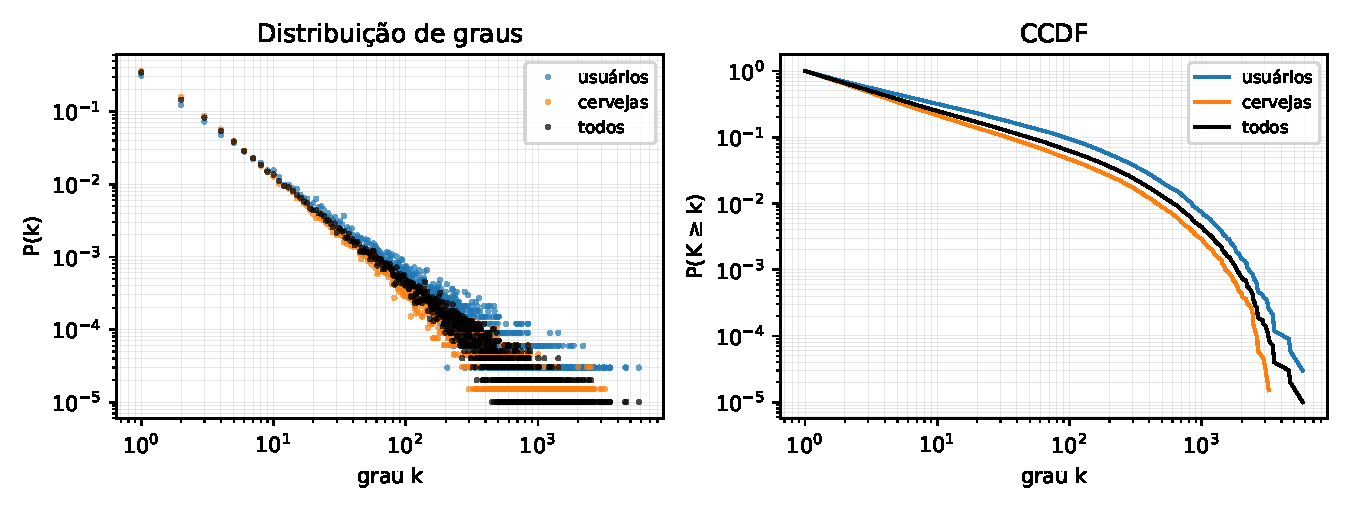
\includegraphics[width=\linewidth]{../results/figures/distribuicao_graus.pdf}
\caption{Distribuição de graus $P(k)$ e CCDF $P(K\ge k)$ em escala log-log, para todos os
vértices e separadamente para usuários e cervejas.}
\label{fig:graus}
\end{figure*}

\textbf{Densidade e componentes.} A densidade é $\rho=\Densidade$. Mesmo em relação ao máximo
possível num grafo bipartido ($|U||B|$ arestas), ela é só $\DensidadeBip$. O grafo tem
\NComponentes{} componentes: a MCC, com \MCCVertices{} vértices (\MCCPercent{} do total), e
\NCompPequenas{} componentes de tamanho 2, cada uma formada por um usuário que avaliou uma única
cerveja que ninguém mais avaliou.

\textbf{Distâncias.} Na MCC, o diâmetro é \Diametro{}, o raio é \Raio{} e o comprimento médio
exato é \LExato{}. Como o grafo é bipartido, distâncias entre usuário e cerveja são ímpares e
distâncias entre vértices do mesmo lado são pares. Pela Figura~\ref{fig:dist}, \FracDistAteQuatro{}
dos pares ordenados da MCC estão a no máximo 4 passos.

\begin{figure}[t]
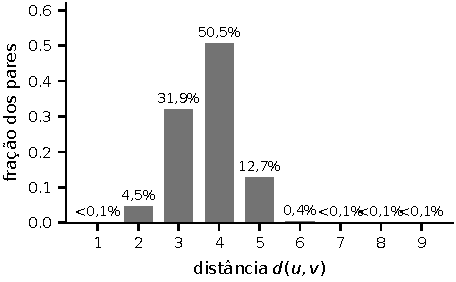
\includegraphics[width=\linewidth]{../results/figures/distribuicao_distancias.pdf}
\caption{Distribuição exata das distâncias entre os pares de vértices da MCC.}
\label{fig:dist}
\end{figure}

\textbf{Triângulos e clusterização.} A contagem exata dá \Triangulos{} triângulos e $C=\Clusterizacao$.
Isso decorre da estrutura: verificamos por BFS (2-coloração) que o grafo é bipartido, e grafos
bipartidos não têm ciclos ímpares, logo não têm triângulos. O cálculo serve como conferência da
implementação, não como achado.

\textbf{Visualização.} A Figura~\ref{fig:viz} mostra um subgrafo de \VizVertices{} vértices obtido
pela ordem da BFS a partir de um vértice sorteado. O grafo inteiro ($\sim\!10^5$ vértices e
$1{,}6\times10^6$ arestas) não seria legível.

\begin{figure}[t]
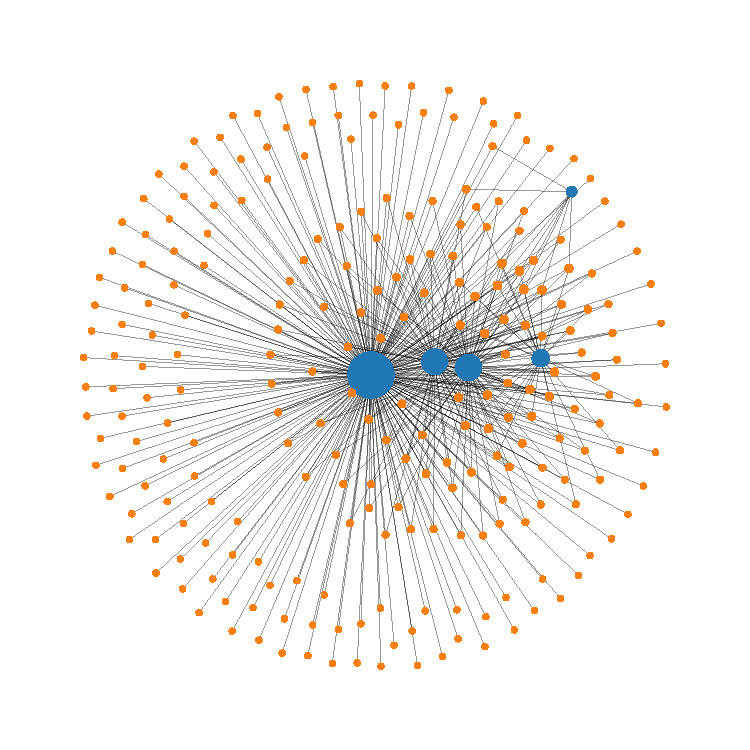
\includegraphics[width=.9\linewidth]{../results/figures/visualizacao_amostra.pdf}
\caption{Visualização reduzida: \VizVertices{} vértices e \VizArestas{} arestas; tamanho
proporcional ao grau no subgrafo. Poucos usuários ligam muitas cervejas.}
\label{fig:viz}
\end{figure}

\subsection{Parte II -- Algoritmos}

\begin{table}[t]
\caption{Parte II: resultado de cada algoritmo na MCC ($|V|=99.356$, $|E|=1.571.439$).}
\label{tab:p2res}
\small
\begin{tabular}{lp{5.4cm}}
\toprule
Algoritmo & Resultado \\
\midrule
BFS & origem sorteada: excentricidade 6 \\
DFS & 42 árvores no grafo completo \\
Eulerianidade & não; 62.054 vértices de grau ímpar \\
Dijkstra & mesma origem: dist. máx. 16{,}00, média 5{,}51 \\
Bellman-Ford & sem ciclo negativo; igual a Dijkstra; 5 passadas \\
Floyd-Warshall & só em amostras ($\le 400$ vértices) \\
Tarjan & 7.260 articulações; 34.340 pontes \\
Prim & AGM: 99.355 arestas, peso 177.260{,}33 \\
Kruskal & AGM: 99.355 arestas, peso 177.260{,}33 \\
\bottomrule
\end{tabular}
\end{table}


A Tabela~\ref{tab:p2res} resume os resultados na MCC. No grafo completo, a DFS encontra
\DFSArvores{} árvores e Tarjan (CFC) encontra \TarjanCFC{} componentes fortemente conexas, o que
confirma as \NComponentes{} componentes. O grafo não é euleriano: há \EulerImpares{} vértices de
grau ímpar no grafo e \EulerImparesMCC{} na MCC, e o teorema dos slides exige zero (circuito) ou
dois (caminho). Prim e Kruskal produzem árvores com o mesmo peso, \AGMPeso{}, e $|V|-1$ arestas;
as árvores podem diferir, pois há muitas arestas de mesmo peso (as notas variam em passos de 0,5).
A partir da origem sorteada, a maior distância ponderada de Dijkstra é \DijkstraMax{} e a média é
\DijkstraMedia{}. Bellman-Ford não encontra ciclo negativo, como esperado com pesos positivos;
com parada antecipada, $d[\,]$ muda em \BFPassadasUteis{} passadas, a seguinte confirma que nada
mais muda, e as distâncias coincidem com as de Dijkstra. Tarjan encontra \TarjanArt{} pontos de
articulação e \TarjanPontes{} pontes, das quais \TarjanPontesFolha{} ligam um vértice de grau 1
ao restante: as pontes são, quase sempre, a única avaliação de um usuário ou de uma cerveja.

\begin{table}[t]
\caption{Tempo real na MCC: média, desvio padrão (DP) e IC de 95\% (Z para $R=30$; t-Student para $R=10$).}
\label{tab:p2tempo}
\footnotesize
\begin{tabular}{@{}lrrrc@{}}
\toprule
Algoritmo & $R$ & Média (s) & DP (s) & IC 95\% (s) \\
\midrule
BFS & 30 & 0{,}137 & 0{,}023 & [0{,}129; 0{,}145] \\
DFS & 30 & 0{,}497 & 0{,}059 & [0{,}476; 0{,}518] \\
Eulerianidade & 30 & 0{,}137 & 0{,}016 & [0{,}131; 0{,}143] \\
Tarjan (art./pontes) & 30 & 0{,}766 & 0{,}047 & [0{,}749; 0{,}783] \\
Tarjan (CFC) & 30 & 0{,}912 & 0{,}046 & [0{,}896; 0{,}929] \\
Dijkstra & 30 & 0{,}674 & 0{,}032 & [0{,}663; 0{,}686] \\
Prim & 30 & 0{,}717 & 0{,}035 & [0{,}705; 0{,}730] \\
Kruskal & 30 & 0{,}753 & 0{,}059 & [0{,}732; 0{,}775] \\
Bellman-Ford$^{*}$ & 10 & 1{,}686 & 0{,}036 & [1{,}660; 1{,}712] \\
\bottomrule
\multicolumn{5}{@{}l}{\footnotesize $^{*}$ com parada antecipada.}
\end{tabular}
\end{table}


As Tabelas~\ref{tab:p2tempo} e~\ref{tab:p2amostras} e a Figura~\ref{fig:desempenho} mostram os
tempos. Uma BFS na MCC leva \TempoBFS{} s e Dijkstra \TempoDijkstra{} s, \RazaoDijkstraBFS{}
vezes mais: o fator $\log V$ explica só parte da diferença; o resto é a constante do
\texttt{heapq}. Na Tabela~\ref{tab:p2exp}, as inclinações contra o custo teórico ficam entre
\ExpMin{} e \ExpMax{} nos algoritmos quase lineares quando ajustadas sobre as médias, e entre
\ExpRepMin{} e \ExpRepMax{} quando ajustadas sobre cada repetição: o tempo cresce
aproximadamente na proporção do custo teórico. A exceção é Kruskal sobre as médias
(\ExpKruskal{}): seu custo por unidade de $E\log V$ cai de \KruskalNsMaior{} ns na menor amostra
para \KruskalNsMCC{} ns na MCC (causa não investigada), mas, por repetição, a inclinação é
\ExpKruskalRep{}. Os subgrafos amostrados por BFS são mais densos que a MCC, pois a BFS alcança
cedo os vértices de grau alto; por isso a inclinação contra $|V|$ isolado (última coluna) é menor
que 1 nos quase lineares e próxima de 3 em Bellman-Ford (\ExpBFV{}). Contra $VE$, Bellman-Ford tem
inclinação \ExpBF{} (\ExpBFRep{} por repetição), e Floyd-Warshall tem \ExpFW{} contra $V^3$, de
acordo com a teoria.

Nos subgrafos de Bellman-Ford, o desvio padrão é grande e o limite inferior do IC chega a ser
negativo (Tabela~\ref{tab:p2amostras}): o tempo é proporcional a $VE$, e $|E|$ varia muito entre
as amostras de mesmo $k$. Com tempos tão assimétricos, o IC pela t-Student, que supõe
normalidade, é pouco informativo; a comparação com a teoria usa, então, a inclinação por
repetição, que considera o $|E|$ de cada amostra.

\begin{table}[t]
\caption{Inclinação de $\log(\text{tempo})$ contra $\log f(V,E)$ (custo teórico; esperado $\approx 1$), ajustada sobre as médias por tamanho e sobre cada repetição do experimento B, e contra $\log V$ (médias).}
\label{tab:p2exp}
\footnotesize
\begin{tabular}{@{}llrrr@{}}
\toprule
Algoritmo & $f(V,E)$ & médias & repetições & vs.\ $V$ \\
\midrule
BFS & $V+E$ & 1{,}18 & 0{,}90 & 0{,}88 \\
DFS & $V+E$ & 1{,}06 & 0{,}97 & 0{,}79 \\
Eulerianidade & $V+E$ & 1{,}13 & 0{,}82 & 0{,}85 \\
Tarjan (art./pontes) & $V+E$ & 1{,}09 & 1{,}00 & 0{,}81 \\
Tarjan (CFC) & $V+E$ & 1{,}15 & 1{,}04 & 0{,}86 \\
Dijkstra & $(V+E)\log V$ & 1{,}03 & 0{,}88 & 0{,}88 \\
Prim & $E\log V$ & 1{,}06 & 0{,}82 & 0{,}89 \\
Kruskal & $E\log V$ & 0{,}76 & 1{,}00 & 0{,}61 \\
Bellman-Ford & $VE$ & 1{,}06 & 1{,}02 & 3{,}03 \\
Floyd-Warshall & $V^3$ & 1{,}00 & 1{,}00 & 3{,}00 \\
\bottomrule
\end{tabular}
\end{table}


\begin{figure*}[t]
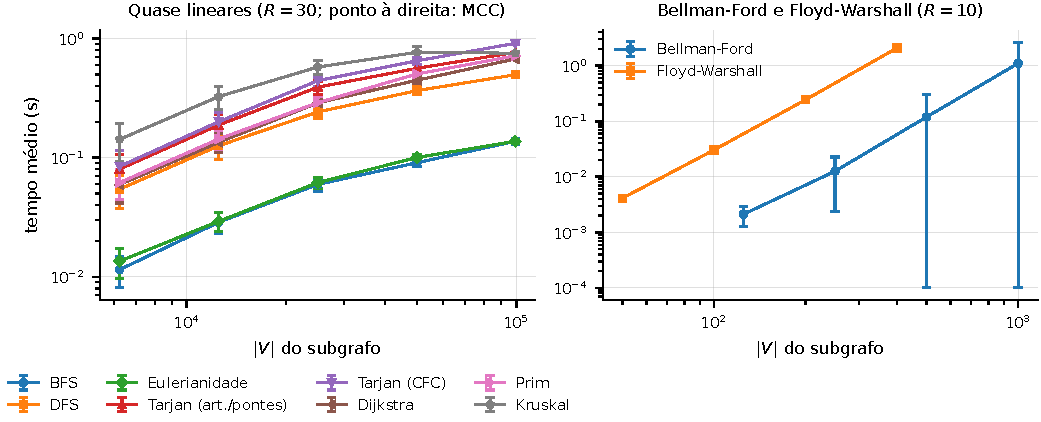
\includegraphics[width=\linewidth]{../results/figures/desempenho.pdf}
\caption{Tempo médio em função de $|V|$ do subgrafo, em escala log-log; barras: IC de 95\%
(limites inferiores negativos de Bellman-Ford foram cortados na escala logarítmica). No painel
esquerdo, o ponto mais à direita de cada curva é a MCC inteira (experimento A).}
\label{fig:desempenho}
\end{figure*}

\begin{table*}[t]
\caption{Experimento B: tempo real em subgrafos conexos de tamanho alvo $k$ (uma amostra nova por repetição; o subgrafo tem exatamente $|V|=k$ vértices). $|E|$ é a média sobre as repetições, com o intervalo de $|E|$ entre parênteses nos algoritmos caros; IC de 95\% pela Normal ($R=30$) ou pela t-Student com $R-1$ graus de liberdade ($R=10$, em Bellman-Ford e Floyd-Warshall). Tempos em segundos.}
\label{tab:p2amostras}
\footnotesize
\setlength{\tabcolsep}{2.2pt}
\begin{tabular}{@{}lrrrrr@{\hspace{0.8em}}lrrrrr@{}}
\toprule
Algoritmo & $k$ & $|E|$ & Média & DP & IC 95\% & Algoritmo & $k$ & $|E|$ & Média & DP & IC 95\% \\
\midrule
BFS & 6.250 & 210.447 & 0{,}011 & 0{,}010 & [0{,}008; 0{,}015] & Dijkstra & 6.250 & 210.447 & 0{,}059 & 0{,}050 & [0{,}042; 0{,}077] \\
BFS & 12.500 & 506.777 & 0{,}029 & 0{,}016 & [0{,}023; 0{,}034] & Dijkstra & 12.500 & 506.777 & 0{,}134 & 0{,}069 & [0{,}110; 0{,}159] \\
BFS & 25.000 & 968.780 & 0{,}060 & 0{,}021 & [0{,}052; 0{,}067] & Dijkstra & 25.000 & 968.780 & 0{,}289 & 0{,}087 & [0{,}258; 0{,}320] \\
BFS & 50.000 & 1.311.116 & 0{,}091 & 0{,}016 & [0{,}085; 0{,}097] & Dijkstra & 50.000 & 1.311.116 & 0{,}447 & 0{,}068 & [0{,}423; 0{,}471] \\
DFS & 6.250 & 210.447 & 0{,}054 & 0{,}047 & [0{,}037; 0{,}071] & Prim & 6.250 & 210.447 & 0{,}062 & 0{,}048 & [0{,}045; 0{,}079] \\
DFS & 12.500 & 506.777 & 0{,}126 & 0{,}080 & [0{,}097; 0{,}155] & Prim & 12.500 & 506.777 & 0{,}144 & 0{,}075 & [0{,}117; 0{,}170] \\
DFS & 25.000 & 968.780 & 0{,}242 & 0{,}077 & [0{,}215; 0{,}270] & Prim & 25.000 & 968.780 & 0{,}290 & 0{,}079 & [0{,}262; 0{,}318] \\
DFS & 50.000 & 1.311.116 & 0{,}366 & 0{,}074 & [0{,}339; 0{,}392] & Prim & 50.000 & 1.311.116 & 0{,}505 & 0{,}095 & [0{,}471; 0{,}539] \\
Eulerianidade & 6.250 & 210.447 & 0{,}014 & 0{,}011 & [0{,}010; 0{,}017] & Kruskal & 6.250 & 210.447 & 0{,}143 & 0{,}140 & [0{,}093; 0{,}193] \\
Eulerianidade & 12.500 & 506.777 & 0{,}029 & 0{,}014 & [0{,}024; 0{,}034] & Kruskal & 12.500 & 506.777 & 0{,}326 & 0{,}204 & [0{,}253; 0{,}399] \\
Eulerianidade & 25.000 & 968.780 & 0{,}062 & 0{,}018 & [0{,}055; 0{,}068] & Kruskal & 25.000 & 968.780 & 0{,}577 & 0{,}214 & [0{,}500; 0{,}653] \\
Eulerianidade & 50.000 & 1.311.116 & 0{,}101 & 0{,}017 & [0{,}095; 0{,}107] & Kruskal & 50.000 & 1.311.116 & 0{,}767 & 0{,}241 & [0{,}681; 0{,}854] \\
Tarjan (art./pontes) & 6.250 & 210.447 & 0{,}080 & 0{,}075 & [0{,}053; 0{,}107] & Bellman-Ford & 125 & 198 (124--531) & 0{,}0021 & 0{,}0011 & [0{,}0013; 0{,}0029] \\
Tarjan (art./pontes) & 12.500 & 506.777 & 0{,}188 & 0{,}116 & [0{,}146; 0{,}230] & Bellman-Ford & 250 & 668 (249--2.627) & 0{,}0126 & 0{,}0142 & [0{,}0024; 0{,}0227] \\
Tarjan (art./pontes) & 25.000 & 968.780 & 0{,}391 & 0{,}138 & [0{,}342; 0{,}440] & Bellman-Ford & 500 & 2.704 (499--17.513) & 0{,}1193 & 0{,}2544 & [-0{,}0627; 0{,}3013] \\
Tarjan (art./pontes) & 50.000 & 1.311.116 & 0{,}563 & 0{,}115 & [0{,}522; 0{,}604] & Bellman-Ford & 1.000 & 9.386 (999--47.735) & 1{,}1005 & 2{,}1322 & [-0{,}4248; 2{,}6257] \\
Tarjan (CFC) & 6.250 & 210.447 & 0{,}085 & 0{,}083 & [0{,}055; 0{,}114] & Floyd-Warshall & 50 & 100 (49--176) & 0{,}0041 & 0{,}0005 & [0{,}0037; 0{,}0045] \\
Tarjan (CFC) & 12.500 & 506.777 & 0{,}200 & 0{,}111 & [0{,}161; 0{,}240] & Floyd-Warshall & 100 & 248 (99--778) & 0{,}0304 & 0{,}0048 & [0{,}0269; 0{,}0338] \\
Tarjan (CFC) & 25.000 & 968.780 & 0{,}443 & 0{,}136 & [0{,}395; 0{,}492] & Floyd-Warshall & 200 & 590 (199--1.554) & 0{,}2430 & 0{,}0170 & [0{,}2309; 0{,}2551] \\
Tarjan (CFC) & 50.000 & 1.311.116 & 0{,}650 & 0{,}135 & [0{,}602; 0{,}699] & Floyd-Warshall & 400 & 902 (399--3.900) & 2{,}0817 & 0{,}1492 & [1{,}9750; 2{,}1884] \\
\bottomrule
\end{tabular}
\end{table*}


Floyd-Warshall e Bellman-Ford não foram executados na MCC na forma do slide. Floyd-Warshall
gastou cerca de \FWnsOp{} ns por iteração do laço interno nos subgrafos medidos; as
$|V|^3 \approx 9{,}8\times10^{14}$ iterações da MCC levariam cerca de \EstFWAnos{} ano(s),
supondo esse custo constante, e só a matriz $|V|\times|V|$ ocuparia pelo menos \EstFWMemGB{} GB
(8 bytes por entrada), contra 15,7 GB de RAM. Para Bellman-Ford, medimos na própria MCC o tempo de
uma passada sobre os $2|E|$ arcos: \BFTempoPassada{} s em média. A versão do slide faz $|V|-1$
passadas mais a verificação de ciclo negativo, o que daria cerca de \EstBFHoras{} h por execução,
e o experimento pede repetições. Na MCC usamos, então, a parada antecipada, que dá o mesmo
resultado: nas \BFOrigens{} origens sorteadas, $d[\,]$ mudou em apenas \BFPassadasFaixa{}
passadas.

\subsection{Parte III -- Análise estrutural}

\textbf{1) Small-world.} A Tabela~\ref{tab:sw} compara o grafo com os modelos. O comprimento médio
$L=\LExato$ (na MCC) é da mesma ordem que o de um grafo aleatório equivalente
($L_{\text{ER}}\approx\LERformula$ pela fórmula e \LERsim{} na instância gerada), o que satisfaz o
primeiro critério do Apêndice A. O segundo critério ($C \gg C_{\text{ER}}$) não se verifica: $C=0$
porque o grafo é bipartido, e $C_{\text{ER}}\approx\CERformula$. Pela definição do enunciado,
portanto, o grafo \textbf{não} é \textit{small-world}. Essa resposta, porém, vem da modelagem, e
não da falta de agrupamento local. Com a medida bipartida, o agrupamento médio $cc_\bullet$ do
grafo (\LatapyG{}) é \LatapyRazao{} vezes o do grafo bipartido aleatório com os mesmos graus
(\LatapyR{}), e os ICs não se sobrepõem. O comprimento médio do grafo real é \RazaoL{} vezes o do
modelo nulo (\LBipR{}). O índice análogo ao $\sigma$ de Humphries e Gurney~\cite{humphries2008},
$\sigma_{\text{bip}}=(cc_\bullet/cc_\bullet^{\text{nulo}})/(L/L^{\text{nulo}})=\SigmaBip$, é maior
que 1: na versão bipartida, a rede combina distâncias curtas com agrupamento acima do acaso.
Faz sentido no domínio: usuários tendem a avaliar conjuntos de cervejas mais parecidos entre si
do que o acaso preveria (o motivo, como preferência por estilos, não foi testado aqui), e poucos
usuários muito ativos e
cervejas muito populares encurtam os caminhos. Na prática, dentro da MCC (\MCCPercent{} dos
vértices), qualquer cerveja está a poucos passos de qualquer usuário, o que favorece, por exemplo,
recomendações baseadas em vizinhança de 2 ou 3 passos.

\begin{table}[t]
\caption{Small-world. $L$: grafo real exato (MCC); modelos clássicos estimados com 200 origens de BFS; nulo bipartido: média de 10 instâncias (100 origens cada). $cc_\bullet$: agrupamento bipartido médio em 2.000 vértices sorteados. Entre colchetes, IC de 95\%.}
\label{tab:sw}
\footnotesize
\begin{tabular}{@{}lllr@{}}
\toprule
Grafo & $L$ & $C$ & grau máx. \\
\midrule
BeerAdvocate & 3{,}725 & 0{,}0 & 5.782 \\
ER (fórmula) & 3{,}332 & $3{,}18\times 10^{-4}$ & -- \\
Erd\H{o}s--Rényi & 3{,}708 & 0{,}0003 & 57 \\
Barabási--Albert ($m_0$=16) & 3{,}261 & 0{,}0025 & 2.024 \\
Watts--Strogatz ($k$=32, $p$=0,1) & 4{,}643 & 0{,}5306 & 41 \\
Nulo bipartido (trocas) & 3{,}672 & 0 & 5.782 \\
\midrule
\multicolumn{4}{@{}l@{}}{$cc_\bullet$ BeerAdvocate: 0{,}0599 [0{,}0567; 0{,}0632]} \\
\multicolumn{4}{@{}l@{}}{$cc_\bullet$ nulo bipartido: 0{,}0306 [0{,}0304; 0{,}0307]} \\
\multicolumn{4}{@{}l@{}}{$L$ do nulo bipartido: IC [3{,}650; 3{,}693]; $\sigma_{\text{bip}} = 1{,}93$} \\
\bottomrule
\end{tabular}
\end{table}


\textbf{2) Lei de potência.} A CCDF (Figura~\ref{fig:pl}) é aproximadamente reta até
$k\approx 10^2$ e depois cai mais rápido. O ajuste exato dá $\hat\gamma=\GammaTodos$
($k_{\min}=\KminTodos$; usuários $\GammaU$, cervejas $\GammaB$), igual ao do \texttt{powerlaw}
até a terceira casa decimal (Tabela~\ref{tab:pl}). A resposta à pergunta do enunciado tem duas
partes. Quanto à \textbf{qualidade absoluta}, a lei de potência é \textbf{rejeitada}: nos três
grupos, nenhum dos \BBoot{} conjuntos sintéticos teve distância KS tão grande quanto a dos dados
($p = 0$, isto é, $p < 1/B = \PBootLimite$). Com quase $10^5$ vértices, o teste detecta desvios pequenos, e o desvio aqui
não é pequeno: $D=\KSTodos$ nos dados, contra no máximo \KSSintMax{} nos conjuntos sintéticos.
Quanto à \textbf{comparação relativa}, a lei de potência é muito mais plausível que a
exponencial, mas a lei de potência truncada e a lognormal se ajustam melhor ($R<0$). Concluímos
que a distribuição tem cauda pesada e \textit{hubs}, como descreve o Apêndice B, mas não segue
uma lei de potência pura: há um corte para graus altos, compatível com o limite prático de quantas
cervejas um usuário avalia e de quantas avaliações uma cerveja recebe em cerca de 15 anos de
dados. Os valores $\hat\gamma<2$ ficam abaixo da faixa $2<\gamma<3$ comum em redes livres de
escala; como $k_{\min}$ é pequeno, o ajuste é determinado sobretudo pelo corpo da distribuição.

\begin{figure*}[t]
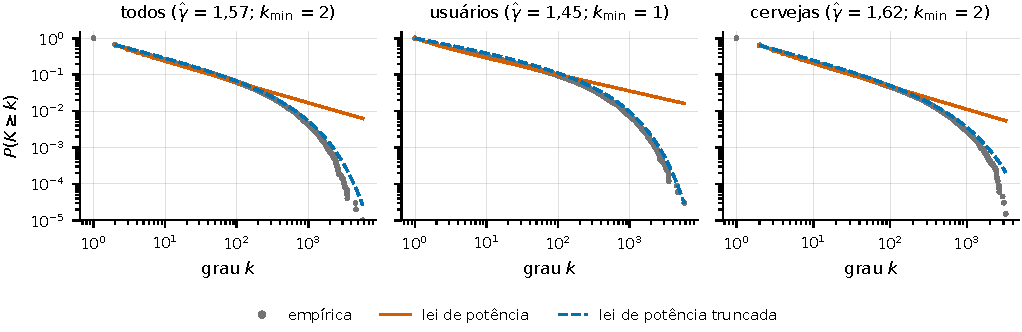
\includegraphics[width=\linewidth]{../results/figures/lei_potencia.pdf}
\caption{CCDF empírica (cinza), lei de potência discreta ajustada a partir de $k_{\min}$
(vermelho) e lei de potência truncada (azul, tracejada), para todos os vértices, usuários e
cervejas.}
\label{fig:pl}
\end{figure*}

\begin{table}[t]
\caption{Ajuste de lei de potência ($\hat\gamma \pm$ erro padrão) e razão de verossimilhança normalizada $R$ (lei de potência vs.\ alternativa; $R<0$ favorece a alternativa).}
\label{tab:pl}
\small
\begin{tabular}{lrrr}
\toprule
 & Todos & Usuários & Cervejas \\
\midrule
$\hat\gamma$ & 1{,}554 $\pm$ 0{,}002 & 1{,}474 $\pm$ 0{,}003 & 1{,}638 $\pm$ 0{,}004 \\
$k_{\min}$ (KS) & 2 & 2 & 3 \\
vértices na cauda & 65.171 & 22.939 & 31.838 \\
distância KS & 0{,}026 & 0{,}051 & 0{,}020 \\
$\alpha$ (\texttt{powerlaw}) & 1{,}565 & 1{,}481 & 1{,}644 \\
$R$ vs.\ exponencial & 94{,}7 & 57{,}0 & 62{,}6 \\
$R$ vs.\ lognormal & -27{,}6 & -25{,}0 & -15{,}5 \\
$R$ vs.\ l.p.\ truncada & -41{,}4 & -32{,}8 & -25{,}7 \\
\bottomrule
\multicolumn{4}{l}{\footnotesize Em todos os testes, $p \le 4{,}4\times 10^{-54}$.}
\end{tabular}
\end{table}


\textbf{3) Robustez.} A Tabela~\ref{tab:rob} e a Figura~\ref{fig:rob} resumem as métricas A--D.
Na remoção aleatória de 5\%, a maior componente mantém $S=\RobSAleat$ dos vértices restantes, o
número de componentes passa de 1 para \RobBAleat{} em média (quase todas são vértices que
perderam seu único vizinho; a fração de isolados é \RobDAleat{}) e a distância média
praticamente não muda (\RobCBase{} sem remoção; \RobCAleat{}, IC \RobCAleatIC{}, após a remoção).
Na remoção dos 5\% de maior grau, $S$ cai para \RobSAlvo{}, surgem \RobBAlvo{} componentes, a
fração de isolados vai a \RobDAlvo{} e a distância média na maior componente sobe para
\RobCAlvo{} (IC \RobCAlvoIC{}). Sendo $c$ o número de componentes, $S_{\text{rand}} \gg
S_{\text{cent}}$ e $c_{\text{cent}} \gg c_{\text{rand}}$: a rede é robusta a falhas aleatórias e
vulnerável a ataques direcionados, o padrão de redes com \textit{hubs} descrito por Albert
et al.~\cite{albert2000}.

\begin{table}[t]
\caption{Robustez na MCC ($n=99.356$, $r=4.968$): remoção aleatória ($T=30$, média $\pm$ DP) e remoção dos $r$ vértices de maior grau. Sem remoção, C é o valor exato; após a remoção, C é estimada por BFS a partir de 100 (aleatória) e 2.000 origens (por grau).}
\label{tab:rob}
\footnotesize
\begin{tabular}{@{}lrrr@{}}
\toprule
Métrica & Sem remoção & Aleatória & Por grau \\
\midrule
A: maior componente & 99.356 & 92.804 $\pm$ 339 & 40.975 \\
A: $S$ & 1{,}0000 & 0{,}9832 $\pm$ 0{,}0036 & 0{,}4341 \\
B: componentes & 1 & 1.577{,}7 $\pm$ 337{,}8 & 52.451 \\
C: distância média & 3{,}725 & 3{,}724 $\pm$ 0{,}044 & 6{,}011 \\
C: maior distância & 9$^{\dagger}$ & 7{,}9 $\pm$ 0{,}4 & 17 \\
D: fração isolados & 0{,}0000 & 0{,}0166 $\pm$ 0{,}0036 & 0{,}5469 \\
\bottomrule
\multicolumn{4}{@{}l}{\footnotesize $^{\dagger}$ diâmetro exato; após a remoção, maior distância vista nas BFS.}
\end{tabular}
\end{table}


\begin{figure*}[t]
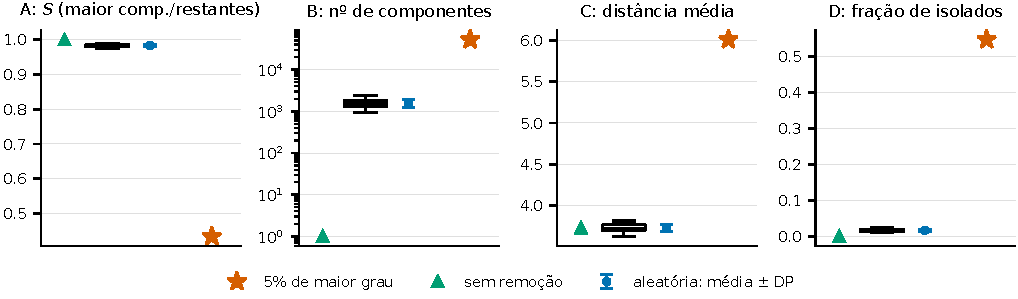
\includegraphics[width=\linewidth]{../results/figures/robustez.pdf}
\caption{Robustez na MCC: boxplots das 30 remoções aleatórias de 5\%, média $\pm$ desvio padrão
(círculo azul), valor após remover os 5\% de maior grau (estrela) e valor sem remoção
(triângulo). O painel B está em escala logarítmica.}
\label{fig:rob}
\end{figure*}

\textbf{4) Descoberta mais interessante.} \Descoberta

\textbf{5) Modelos clássicos (extra).} Nenhum modelo da Tabela~\ref{tab:sw} reproduz o grafo.
Erd\H{o}s--Rényi e Watts--Strogatz têm graus concentrados em torno da média
(Figura~\ref{fig:modelos}) e não têm \textit{hubs}; Watts--Strogatz ainda tem muitos triângulos,
que um grafo bipartido não pode ter. Barabási--Albert~\cite{barabasi1999} é o único dos três com
cauda pesada, mas sua cauda é mais leve que a do grafo real (expoente teórico $\gamma=3$; grau
máximo \GrauMaxBA{} contra \GrauMax{}) e ele não é bipartido. Entre os modelos clássicos, o
Barabási--Albert é o mais próximo na distribuição de graus, mas nenhum deles descreve o grafo;
seria preciso um modelo bipartido com ligação preferencial nos dois lados.

\begin{figure}[t]
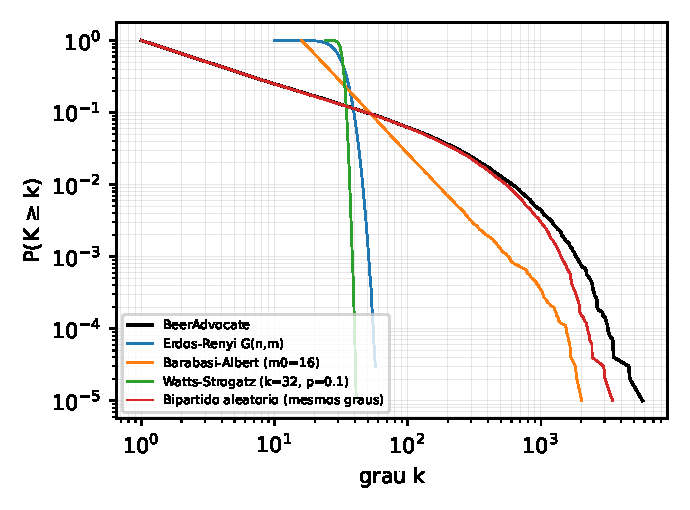
\includegraphics[width=\linewidth]{../results/figures/modelos_ccdf.pdf}
\caption{CCDF de graus do grafo e dos modelos clássicos com o mesmo $n$ e grau médio semelhante.
O nulo bipartido tem, por construção, os mesmos graus do grafo real.}
\label{fig:modelos}
\end{figure}

% ======================================================================
\section{Discussão crítica}\label{sec:discussao}

\textbf{Modelagem.} O grafo bipartido é fiel aos dados, mas torna triviais algumas medidas do
enunciado (triângulos e clusterização), que precisaram ser complementadas pela versão bipartida.
Os pesos $6-\bar o$ são uma convenção: outra escolha mudaria os caminhos mínimos ponderados e a
AGM, mas não as medidas não ponderadas.

\textbf{Dados.} O conjunto foi retirado de circulação a pedido do BeerAdvocate, e o SNAP não
declara licença; isso limita a reprodução por terceiros. Registramos o SHA-256 do arquivo usado.
O número de avaliações difere em 355 do informado pelo SNAP, e \NAvSemUsuario{} avaliações sem nome
de usuário foram descartadas.

\textbf{Desempenho.} As medições foram feitas em Python puro, num notebook, com outros processos
do sistema ativos; os valores absolutos refletem o interpretador, e não só o algoritmo. As
amostras por BFS não são subgrafos ``típicos'': ficam mais densas que a MCC, o que mistura o
efeito de $V$ e de $E$; por isso a comparação foi feita contra $f(V,E)$. As estimativas para
Floyd-Warshall e Bellman-Ford na MCC supõem custo constante por operação; efeitos de memória
\textit{cache} tendem a torná-las otimistas.

\textbf{Aproximações.} São estimativas, e não valores exatos: $L$ dos modelos (200 origens; 100
por instância do nulo bipartido), a distância média após as remoções (100 ou \RobKAlvo{} origens) e
$cc_\bullet$ (amostra de \LatapyAmostra{} vértices). Para cada uma reportamos o IC. O comprimento
médio, o diâmetro e o raio da MCC real são exatos.

% ======================================================================
\section{Conclusão}\label{sec:conclusao}

Construímos o grafo bipartido usuário--cerveja do \textit{web-BeerAdvocate}, com \NVertices{}
vértices e \NArestas{} arestas, e calculamos todas as medidas da Parte I. Os algoritmos da Parte II
foram implementados conforme os slides, validados contra o NetworkX e medidos com intervalos de
confiança; os tempos crescem de forma compatível com as complexidades teóricas. O grafo é muito
esparso e quase todo contido numa componente gigante, com distâncias curtas (diâmetro
\Diametro{}, $L=\LExato$) e agrupamento bipartido acima do acaso. A distribuição de graus tem
cauda pesada, mas não é uma lei de potência pura. A conectividade depende de poucos
\textit{hubs}: a rede resiste à remoção aleatória de 5\% dos vértices, mas se fragmenta quando os
5\% de maior grau são removidos. Como trabalho futuro, pode-se estudar a evolução temporal das
avaliações.

\section*{Disponibilidade}
Código, dados tratados, resultados e instruções de execução: \url{\LinkRepositorio}.

\section*{Uso de inteligência artificial}
\DeclaracaoIA

\bibliographystyle{ACM-Reference-Format}
\bibliography{referencias}

\end{document}
